\documentclass[11pt]{article}
\usepackage[margin=1in]{geometry}
\usepackage{amsmath,amssymb,amsthm}
\usepackage{graphicx}
\usepackage[hidelinks]{hyperref}

\newtheorem{theorem}{Theorem}
\newtheorem{corollary}{Corollary}
\newtheorem{remark}{Remark}

\newcommand{\BFPP}{\mathrm{BFPP}}
\newcommand{\K}{\mathbb K}

\title{Ordinal compacta and the ball fixed point property for \(C(K,p)\)}
\author{arXiv automatic math run \texttt{fa\_banach\_001}}
\date{2026-06-14}

\begin{document}
\maketitle

\section*{Source Question}

The source paper is Aviles--Japon--Lennard--Martinez-Cervantes--Stawski,
\emph{The ball fixed point property in spaces of continuous functions},
arXiv:2506.17995 \cite{source}.  A Banach space has the ball fixed point
property, abbreviated \(\BFPP\), if every nonexpansive self-map of its closed
unit ball has a fixed point.

The final list of questions asks in item (i) whether there is an infinite
compact \(K\) and a non-isolated \(p\in K\) such that \(C(K,p)\) has the
\(\BFPP\), where \(C(K,p)=\{f\in C(K):f(p)=0\}\).

\begin{center}
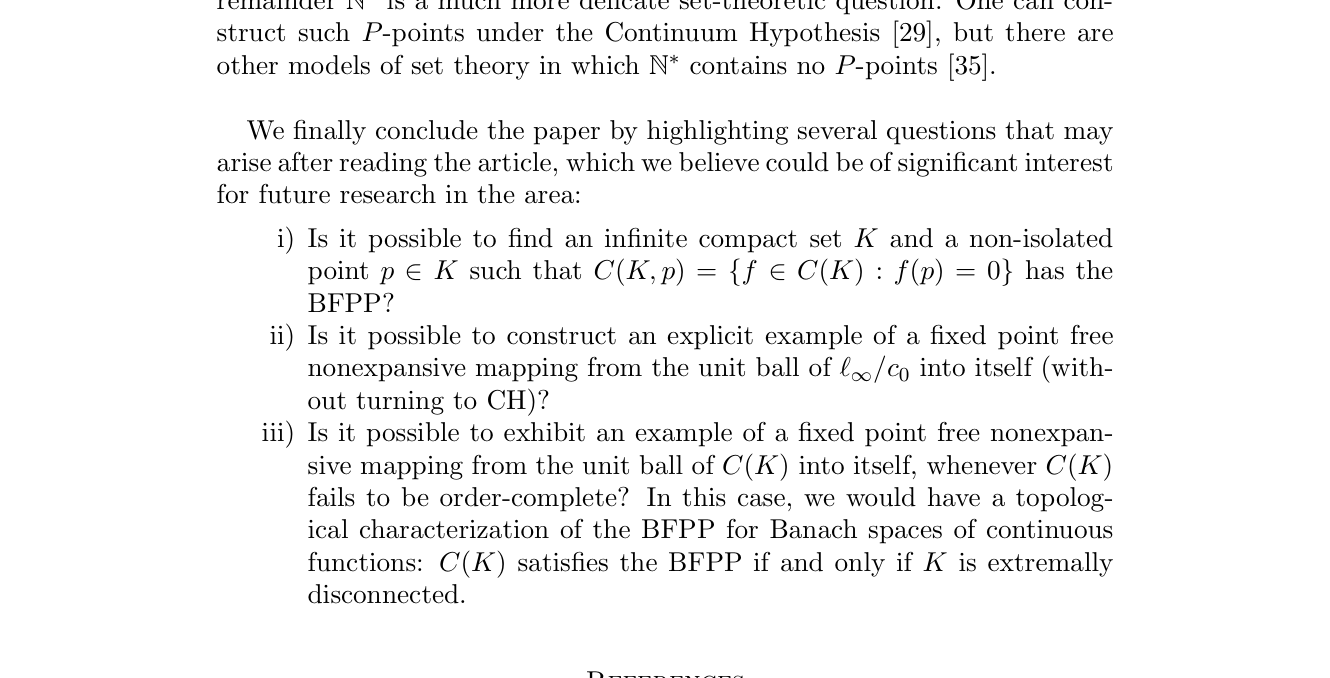
\includegraphics[width=\linewidth]{figures/open_question_i_crop.png}
\end{center}

\section*{Idea of the Proof}

For \(K=[0,\kappa]\) and \(p=\kappa\), the space \(C(K,p)\) consists of
continuous scalar functions on the compact ordinal interval that vanish at the
endpoint.  A one-step ordinal shift places the value \(1\) at \(0\), shifts
successor values forward, leaves limit-ordinal values unchanged, and keeps the
endpoint value \(0\).  This map is nonexpansive.  Any fixed point would have
to be \(1\) at \(0\), hence \(1\) at every successor ordinal, and then by
continuity \(1\) at every limit ordinal below \(\kappa\).  That contradicts
continuity at the endpoint \(\kappa\), where functions in \(C(K,p)\) vanish.

\section*{Partial Result}

\begin{theorem}\label{thm:ordinal}
Let \(\kappa\) be a nonzero limit ordinal, let \(K=[0,\kappa]\) with the order
topology, and let \(p=\kappa\).  Then \(C(K,p)\) fails the ball fixed point
property.
\end{theorem}

\begin{proof}
Let
\[
  X=C(K,p)=\{f\in C([0,\kappa]): f(\kappa)=0\}
\]
with the supremum norm.  Define \(T:B_X\to B_X\) by
\[
(Tf)(\alpha)=
\begin{cases}
1, & \alpha=0,\\
f(\beta), & \alpha=\beta+1<\kappa,\\
f(\alpha), & 0<\alpha<\kappa \text{ is a limit ordinal},\\
0, & \alpha=\kappa.
\end{cases}
\]

First we check that \(Tf\in X\).  Successor ordinals are isolated, and \(0\)
is isolated, so continuity is automatic there.  Let \(0<\lambda<\kappa\) be a
limit ordinal.  Since \(f\) is continuous at \(\lambda\), for every
\(\varepsilon>0\) there is \(\gamma<\lambda\) such that
\(|f(\alpha)-f(\lambda)|<\varepsilon\) whenever
\(\gamma<\alpha\le\lambda\).  If \(\alpha\) is a limit ordinal in
\((\gamma,\lambda]\), then \((Tf)(\alpha)=f(\alpha)\); if
\(\alpha=\beta+1\in(\gamma+1,\lambda)\), then
\((Tf)(\alpha)=f(\beta)\), and \(\gamma<\beta<\lambda\).  Thus
\((Tf)(\alpha)\to f(\lambda)=(Tf)(\lambda)\) as \(\alpha\to\lambda\).

At the endpoint \(\kappa\), use \(f(\kappa)=0\).  Given \(\varepsilon>0\),
choose \(\gamma<\kappa\) such that \(|f(\alpha)|<\varepsilon\) for
\(\gamma<\alpha\le\kappa\).  Then \(|(Tf)(\alpha)|<\varepsilon\) for all
sufficiently large \(\alpha<\kappa\), whether \(\alpha\) is a limit ordinal or
a successor ordinal.  Hence \(Tf\) is continuous at \(\kappa\) and
\((Tf)(\kappa)=0\).  Also \(T(B_X)\subset B_X\), because \(Tf\) takes only the
value \(1\), the value \(0\), and values already taken by \(f\).

The map \(T\) is nonexpansive.  For \(f,g\in B_X\), at \(0\) and \(\kappa\)
the difference \((Tf)-(Tg)\) is zero.  At a successor \(\beta+1<\kappa\), it
equals \(f(\beta)-g(\beta)\).  At a nonzero limit ordinal
\(\lambda<\kappa\), it equals \(f(\lambda)-g(\lambda)\).  Therefore
\[
  \|Tf-Tg\|_\infty\le \|f-g\|_\infty .
\]

Finally suppose that \(f\in B_X\) is a fixed point of \(T\).  Then
\(f(0)=1\).  By transfinite induction, \(f(\alpha)=1\) for every
\(\alpha<\kappa\): the successor step follows from
\[
  f(\beta+1)=(Tf)(\beta+1)=f(\beta),
\]
and the limit step follows from continuity.  Since \(\kappa\) is a limit
ordinal, this forces \(\lim_{\alpha\to\kappa}f(\alpha)=1\), contradicting
\(f(\kappa)=0\).  Hence \(T\) is fixed-point-free, and \(X\) fails the
\(\BFPP\).
\end{proof}

\begin{corollary}\label{cor:Ppoint}
For every uncountable regular cardinal \(\kappa\), the compact ordinal
\([0,\kappa]\) has a non-isolated \(P\)-point \(p=\kappa\), yet
\[
  C([0,\kappa],p)
\]
fails the \(\BFPP\).
\end{corollary}

\begin{proof}
The point \(\kappa\) is non-isolated because \(\kappa\) is a limit ordinal.  It
is a \(P\)-point because a countable intersection of neighborhoods of
\(\kappa\) contains an interval \((\gamma,\kappa]\), using
\(\operatorname{cf}(\kappa)>\omega\).  The failure of \(\BFPP\) is
Theorem~\ref{thm:ordinal}.
\end{proof}

\section*{Scope}

This does not answer the source question positively or negatively in full.  It
rules out a large and classical family of candidates, including the standard
compact ordinal with a non-isolated \(P\)-point, \([0,\omega_1]\).  It also
gives an elementary fixed-point-free map independent of the source paper's
cardinal family \(K^{\kappa,\Gamma}\).

\section*{Novelty and verification notes}

The local run indexes were searched for arXiv \texttt{2506.17995}, BFPP,
``ball fixed point property'', \(C(K,p)\), \(P\)-points, and spaces of
continuous functions.  No exact previous packet or attempt for this source
paper was found.  A bounded web search on 2026-06-14 for the same phrases
found the source arXiv page and no later explicit answer to the final
questions.

The only proof point needing care is continuity of \(Tf\) at limit ordinals
and at \(\kappa\).  The definition of \(T\) was chosen exactly so that the
successor-shift values converge to the already-prescribed limit values.

\begin{thebibliography}{9}
\bibitem{source}
A. Aviles, M. Japon, C. Lennard, G. Martinez-Cervantes, A. Stawski,
\emph{The ball fixed point property in spaces of continuous functions},
arXiv:2506.17995, 2025.
\end{thebibliography}

\end{document}
